\chapter{Introducción}

El primer capítulo es siempre una introducción. En ella debes resumir de forma esquemática pero suficientemente clara lo esencial de cada una de las partes del trabajo. La lectura de este primer capítulo ha de dar una primera idea clara de lo que se pretendía, las conclusiones a las que se ha llegado y del procedimiento seguido.

Como tal, es uno de los capítulos más importantes de la memoria. Las ideas principales a transmitir son la identificación del problema a tratar, la justificación de su importancia, los objetivos generales (a grandes rasgos) y un adelanto de la contribución que esperas hacer.

Típicamente una introducción tiene tres apartados: Motivación, Planteamiento del trabajo, Estructura del trabajo. (Texto Normal del menú de estilos.)

(Ejemplo de nota al pie\footnote{Ejemplo de nota al pie.}.)

\section{Motivación/justificación del tema a tratar}

¿Cuál es el problema que quieres tratar?

¿Cuáles crees que son las causas?

¿Por qué es relevante el problema?

A continuación, se indica con un ejemplo cómo deben introducirse los títulos y las fuentes en Tablas y Figuras.

\begin{table}[t]
	\begin{center}
	\caption{Ejemplo de tabla con sus principales elementos.}
	\label{tab:tab-1}
	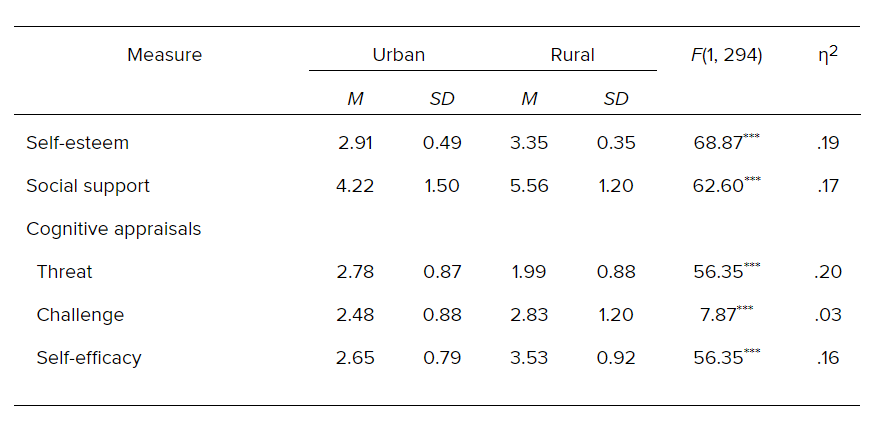
\includegraphics[width=4.90737in,height=2.42708in]{tabla}

	\small Fuente: American Psychological Association, 2020e.
	\end{center}
\end{table}

\begin{figure}[ht]
	\begin{center}
		\caption{Ejemplo de figura realizada para nuestro trabajo.}
		\label{fig:fig-1}
		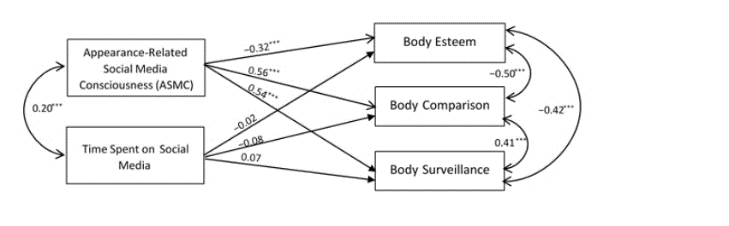
\includegraphics[width=4.90737in,height=2.42708in]{figura}

		\small Fuente: American Psychological Association, 2020f.
	\end{center}
\end{figure}

\section{Planteamiento del trabajo/problema}

¿Cómo se podría solucionar el problema?

¿Qué es lo que se propone?

Aquí describes tu objetivo en términos generales.

\section{Estructura del trabajo}

Aquí describes brevemente lo que vas a contar en cada uno de los capítulos siguientes.